Tra le due componenti in cui si articola il progetto, la prima sviluppata è stata la componente \emph{client}. Questa parte consiste sostanzialmente di una applicazione per dispositivi \emph{smartphone} Android, completamente riscritta a partire da alcuni sviluppi precedenti per poter assolvere alle nuove funzioni specifiche di \emph{PathS}. Si riassumono i requisiti che sono stati identificati e i criteri principali che hanno determinato lo sviluppo del software. 

\section{Requisiti}
Il client mobile \emph{PathS} presenta tutte le caratteristiche di una applicazione sviluppata secondo il paradigma \emph{Web\textsuperscript{2}}. 
Le funzioni principali che deve svolgere possono essere riassunte in:
\begin{itemize}
\item raccogliere dei valori riguardante l'ambiente circostante tramite i sensore di luminosità e microfono;
\item tenere traccia degli spostamenti effettuati e abbinarli ai relativi campioni;
\item offrire le indicazioni di percorso secondo la destinazione e le modalità richieste dall'utente;
\item cercare di coinvolgere il più possibile l'utente incentivando l'uso dell'applicazione.
\end{itemize}

Alcuni di questi requisiti possono essere identificati come \emph{funzionali} e sono indispensabili per gli scopi generali del progetto. Le operazioni di campionamento tramite i sensori ambientali e il tracciamento della posizione tramite GPS sono gli elementi fondamentali richiesti per poter disporre dei dati necessari alle successive elaborazioni. Tuttavia nessun utente finale sarebbe motivato nell'eseguire queste operazioni se l'applicazione non fornisse una qualche altra utilità. Un gruppo di utenti volontari può essere selezionato per alcune campagne di raccolta, tuttavia per motivare un utilizzatore occasionale era necessario adottare altre strategie. 
Per questo sono stati identificati gli altri due requisiti, così da motivare l'utilizzo dell'applicazione stessa. Si è pensato che fornendo direttamente il servizio di \emph{routing} dallo smartphone, si potevano sfruttare i risultati del servizio ma contemporaneamente contribuire allo stesso raccogliendo ulteriori informazioni durante il percorso. Per rendere ottimali i dati raccolti durante l'uso, era inoltre necessario ideare uno stratagemma affinchè il dispositivo fosse in una condizione ideale per il campionamento. La soluzione è venuta dalla proposta di adottare delle funzioni di \emph{Augmented Reality} (Realtà Aumentata). In questo modo non solo si sarebbe ottenuto un maggiore coinvolgimento dell'utente finale, ma inconsapevolmente l'utilizzatore stesso avrebbe mantenuto lo \emph{smartphone} fuori dalla tasca in condizioni perfette per le misurazioni tramite i sensori.
Seguendo queste indicazioni quindi, si è strutturata una applicazione \emph{Android} composta principalmente di 3 moduli:
\begin{itemize}

\begin{figure}[h]
  \centering
  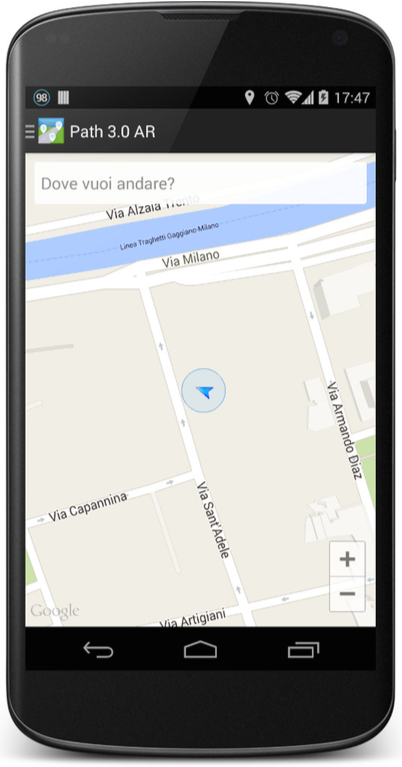
\includegraphics[height=10cm]{app-mappa}
  \caption{\footnotesize{Modalità \emph{Mappa} dell'applicazione mobile PathS.}}
  \label{fig:app-mappa}
\end{figure}

\item \textbf{Mappa}: E' la schermata con la quale l'utente può selezionare una destinazione e visualizzare il percorso suggerito. In questa sezione l'applicazione comunica con i servizi Google per la selezione dei luoghi e la ricerca della destinazione, mentre interroga la componente \emph{server} di \emph{PathS} per richiedere i percorsi da suggerire. Il risultato è visualizzato in una vista a cartina stile Google Maps.

\begin{figure}[h]
  \centering
  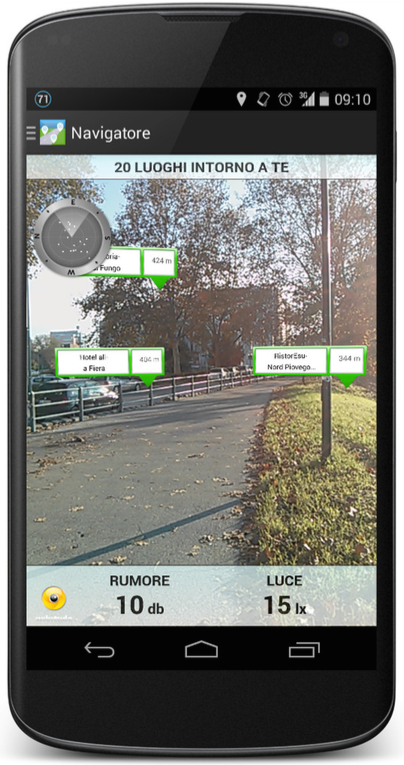
\includegraphics[height=10cm]{app-navigatore}
  \caption{\footnotesize{Modalità \emph{Navigatore} dell'applicazione mobile PathS.}}
  \label{fig:app-navigatore}
\end{figure}

\item \textbf{Navigatore}: E' la modalità con la quale si guida l'utente durante il percorso pedonale: si forniscono le indicazioni di svolta ed altre informazioni aggiuntive presentandole in realtà aumentata. L'utente può quindi mantenere il dispositivo in posizione verticale inquadrando l'orizzonte con la fotocamera e visualizzare in modo ``sovrapposto'' le informazioni di cui necessita. Durante questa modalità sono eseguiti in \emph{background} i campionamenti di rumorosità e luminosità che saranno successivamente inviati al server.
\item \textbf{Impostazioni}: In questa parte dell'applicazione è possibile configurare alcuni parametri di funzionamento e di visualizzazione.
\end{itemize} 

\section{Tecnologie}
Riassunto delle tecnologie adottate per la realizzazione della componente \emph{client}: AndroidSDK, Wikitude.

\section{Stato attuale}
Risultati ottenuti con la parte client. Funzionamento ed eventuali limiti riscontrati.
